\section{Samples}
\label{sec:vhdl-samples}

In order to generate code, port wake events have to be refined to use counters. Two counters \code{lockingCount} and \code{unlockingCount} are introduced. The statemachine WM are refined accordingly, by introducing the transitions that decreased the counter (see Figure~\ref{fig:m3-WM}). The guards of the old transition are refined accordingly using the counters.
\begin{figure}[!htbp]
  \centering
  \ifplastex
  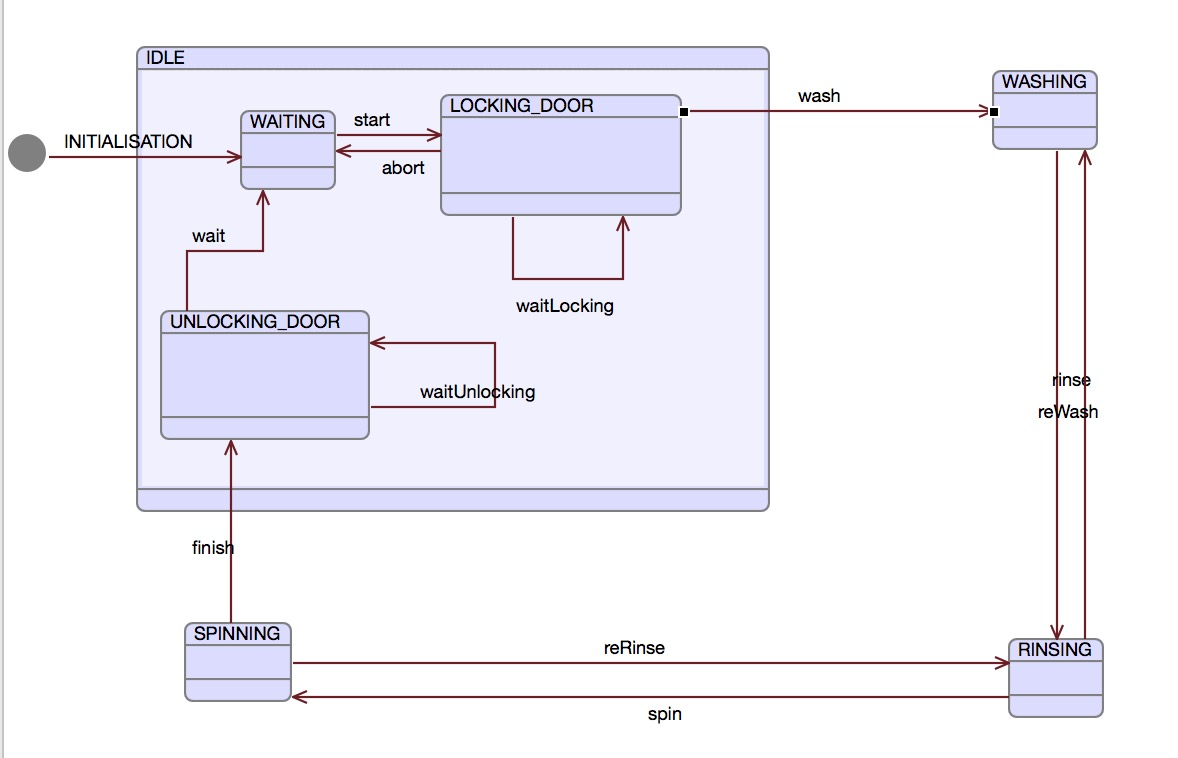
\includegraphics[width=512]{figures/vhdl-WM-m3_WM}
  \else
  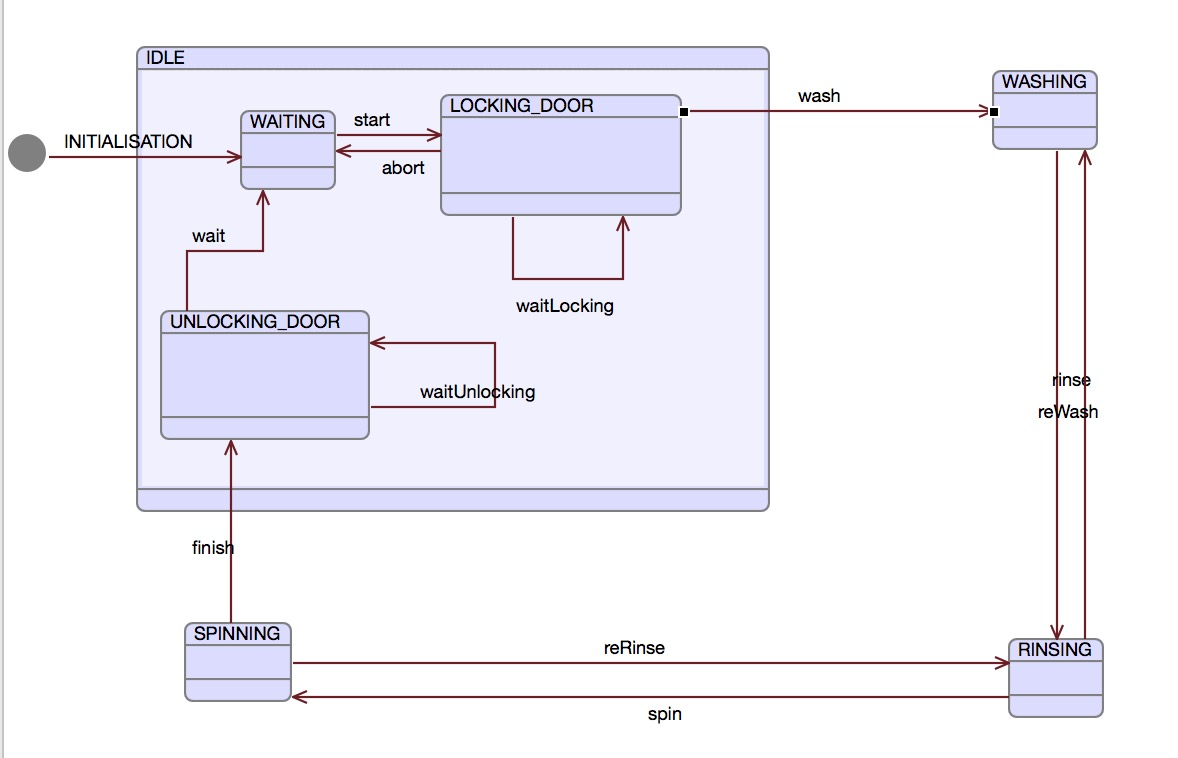
\includegraphics[width=0.5\textwidth]{figures/vhdl-WM-m3_WM}
  \fi
  \caption{Counters in the third refinement of WM}
  \label{fig:m3-WM}
\end{figure}


The following VHDL code is generated for the \code{WM} component of the Washing Machine example.

\begin{verbatim}
LIBRARY ieee;
USE ieee.std_logic_1164.all;
USE ieee.std_logic_unsigned.all;

ENTITY WM IS
  PORT (
    clk : IN std_logic;
    reset : IN std_logic;
    lockedStatus : IN BOOL;
    pID : IN PID;
    lockCommand : OUT BOOL;
    wmStatus : OUT washingMachine_STATES;
  );

  TYPE washingMachine_STATES is (IDLE, WASHING, RINSING, SPINNING);
  TYPE IDLE_sm_STATES is (LOCKING_DOOR, UNLOCKING_DOOR, WAITING, IDLE_sm_NULL);
  TYPE BOOL is (TRUE, FALSE);
  TYPE PID is (noOp, Normal);
  TYPE washingMachine_STATES is (IDLE, WASHING, RINSING, SPINNING);
END WM;

ARCHITECTURE behaviour OF WM IS
  signal locked : BOOL;
  signal unlockingCount : int;
  signal lockingCount : int;
  signal current_washingMachine : washingMachine_STATES;
  signal next_washingMachine : washingMachine_STATES;
  signal current_IDLE_sm : IDLE_sm_STATES;
  signal next_IDLE_sm : IDLE_sm_STATES;
BEGIN

  PROCESS (clk, reset)
  BEGIN
    IF (reset = '1') THEN
      current_IDLE_sm <= WAITING
      current_washingMachine <= IDLE
    ELSIF (raising_edge(clk)) THEN
      current_washingMachine <= next_washingMachine
      current_IDLE_sm <= next_IDLE_sm
    END IF;
  END PROCESS;

  PROCESS (lockedStatus)
  BEGIN
    IF (lockedStatus = TRUE) THEN
      locked <= TRUE
    END IF;
  END PROCESS;

  PROCESS (pID)
  BEGIN
    IF (IDLE_sm ≠ WAITING) THEN
    END IF;
  END PROCESS;

  PROCESS (current_washingMachine, lockedStatus, pID)
  BEGIN
    CASE current_washingMachine IS 
      WHEN IDLE => 
        CASE current_IDLE_sm IS 
          WHEN LOCKING_DOOR => 
            IF (lockingCount = 0) & (locked = FALSE) THEN
              next_IDLE_sm <= WAITING
            ELSIF (lockingCount ≠ 0) THEN
              lockingCount   <=   lockingCount − 1
            ELSIF (lockingCount = 0) & (locked = TRUE) THEN
              next_washingMachine <= WASHING
              next_IDLE_sm <= IDLE_sm_NULL
            END IF;
          WHEN UNLOCKING_DOOR => 
            IF (unlockingCount = 0) THEN
              next_IDLE_sm <= WAITING
            ELSIF (unlockingCount ≠ 0) THEN
              unlockingCount   <=   unlockingCount − 1
            END IF;
          WHEN WAITING => 
            IF ((true) & (true)) THEN
              lockingCount   <=   4
              next_IDLE_sm <= LOCKING_DOOR
              lockCommand <= TRUE
            END IF;
      WHEN WASHING => 
        IF ((true) & (true)) THEN
          next_washingMachine <= RINSING
          wmStatus <= RINSING
        END IF;
      WHEN RINSING => 
        IF ((true) & (true)) THEN
          next_washingMachine <= WASHING
          wmStatus <= WASHING
        ELSIF ((true) & (true)) THEN
          next_washingMachine <= SPINNING
          wmStatus <= SPINNING
        END IF;
      WHEN SPINNING => 
        IF ((true) & (true)) THEN
          next_washingMachine <= RINSING
          wmStatus <= RINSING
        ELSIF ((true) & (true)) THEN
          unlockingCount   <=   4
          next_IDLE_sm <= UNLOCKING_DOOR
          next_washingMachine <= IDLE
          locked   <=   FALSE
          lockCommand <= FALSE
          wmStatus <= IDLE
        END IF;
  END PROCESS;
END behaviour
\end{verbatim}

%%% Local Variables:
%%% mode: latex
%%% TeX-master: "vhdl-user_manual"
%%% End:
